% CS.tex

55\chapter{Grille Cubed-Sphère}

\section{Définition géométrique de la Cubed-Sphère}

\subsection{La sphère $\mathbb{S}_a^2$}

Soit $a > 0$ un réel strictement positif. $\mathbb{S}_a^2$ est la sphère de centre $O : (0,0,0) \in \mathbb{R}^3$ et de rayon $a$ :

\begin{equation}
\mathbb{S}_a^2 := \left\lbrace
\mathbf{x} = (x,y,z)^T \in \mathbb{R}^3 \text{ tels que } x^2+y^2+z^2 = a^2
\right\rbrace
\end{equation} 

On nomme grand cercle, un cercle de centre $O$ et de rayon $a$. Un grand cercle est inclus dans la sphère $\mathbb{S}_a^2$.
Soient $C_1$ et $C_2$ deux grands cercles distincts, $\mathbf{x} \in C_1 \cap C_2$ alors $\mathbf{x} \in \mathbb{S}_a^2$.
On pose les points $\mathbf{x}_1 \in C_1$ et $\mathbf{x}_2 \in C_2$, on peut alors définir $\alpha$ (resp. $\beta$) l’abscisse curviligne de $\mathbf{x}$ le long de $C_1$ (resp. $C_2$) avec $\mathbf{x}_1$ (resp. $\mathbf{x}_2$) comme origine (Voir figure \ref{fig: grands cercles}).


\begin{figure}[ht]
\begin{center}
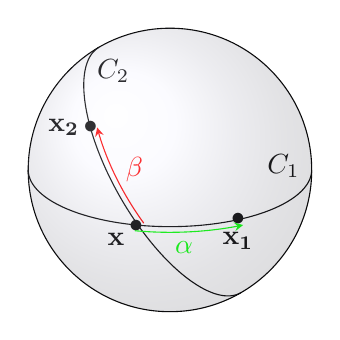
\begin{tikzpicture}[scale=1.8]
	% \draw [color=gray] (-1.5,-1.5) grid[step=0.1] (1.5,1.5);
	\draw [samples=100,domain=0:-180] plot({cos(\x)},{0.4*sin(\x)});
	\draw (0.8,0.03) node {$C_1$} ;  
	\draw [rotate=-60,samples=100,domain=0:-180] plot({cos(\x)},{0.4*sin(\x)});
	\draw (-0.4,0.7) node {$C_2$} ; 
	\draw (-0.24,-0.4) node {$\bullet$} ;
	\draw (-0.38,-0.49) node {$\mathbf{x}$} ;
	\draw (0.48,-0.35) node {$\bullet$} ;
	\draw (0.48,-0.5) node {$\mathbf{x_1}$} ;
	\draw [>=stealth, <-,color=green,domain=-62:-103] plot({1.1*cos(\x)},{0.44*sin(\x)});
	\draw [color=green] (0.1,-0.55) node {$\alpha$} ;
	\draw (-0.56,0.3) node {$\bullet$} ;
	\draw (-0.75,0.3) node {$\mathbf{x_2}$} ;
	\draw [rotate=-60,>=stealth, ->,color=red,domain=-75:-125] plot({0.9*cos(\x)},{0.36*sin(\x)});
	\draw [color=red] (-0.25,0) node {$\beta$} ;
    \draw (0,0) circle (1cm);
    \shade[ball color=blue!10!white,opacity=0.20] (0,0) circle (1cm);
\end{tikzpicture}
\end{center}
\caption{Grands cercles sur la sphère $\mathbb{S}_a^2$ et abscisses curvilignes $\alpha$ et $\beta$.}
\label{fig: grands cercles}
\end{figure}

En tout point $\mathbf{x} \in \mathbb{S}_a^2$, il existe un plan tangent à la sphère noté $\mathbb{T}_{\mathbf{x}}\mathbb{S}_a^2$. Il est engendré par les vecteurs $\mathbf{e}_{\alpha}$ et $\mathbf{e}_{\beta}$ (Voir figure \ref{fig: e_alpha et e_beta}) donnés par :

\begin{equation}
\mathbf{e}_{\alpha} := \dfrac{\partial \mathbf{x}}{\partial \alpha} \text{ et } \mathbf{e}_{\beta} := \dfrac{\partial \mathbf{x}}{\partial \beta}
\end{equation}

\begin{figure}[ht]
\begin{center}
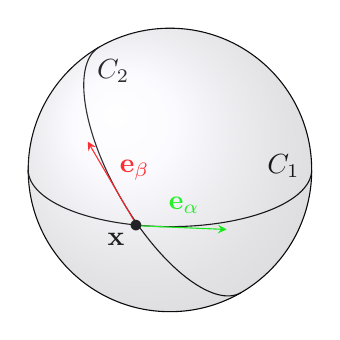
\begin{tikzpicture}[scale=1.8]
	%\draw [color=gray] (-1.5,-1.5) grid[step=0.1] (1.5,1.5);
	\draw [samples=100,domain=0:-180] plot({cos(\x)},{0.4*sin(\x)});
	\draw (0.8,0.03) node {$C_1$} ;  
	\draw [rotate=-60,samples=100,domain=0:-180] plot({cos(\x)},{0.4*sin(\x)});
	\draw (-0.4,0.7) node {$C_2$} ; 
	
	\draw [>=stealth, ->, color=green] (-0.24,-0.393) -- (0.4,-0.42) ;
	\draw [color=green] (0.1,-0.25) node {$\mathbf{e}_{\alpha}$} ;	
	\draw [>=stealth, ->, color=red] (-0.24,-0.38) -- (-0.58,0.20) ;	
	\draw [color=red] (-0.25,0) node {$\mathbf{e}_{\beta}$} ;
	
	\draw (-0.24,-0.4) node {$\bullet$} ;
	\draw (-0.38,-0.49) node {$\mathbf{x}$} ;
	\draw (0,0) circle (1cm);
    \shade[ball color=blue!10!white,opacity=0.20] (0,0) circle (1cm);
\end{tikzpicture}
\end{center}
\caption{Vecteurs $\mathbf{e}_{\alpha}$ et $\mathbf{e}_{\beta}$ associés au cercles $C_1$ et $C_2$ de $\mathbb{S}_a^2$.}
\label{fig: e_alpha et e_beta}
\end{figure}

A partir de ces vecteurs $\mathbf{e}_{\alpha}$ et $\mathbf{e}_{\beta}$, une base duale de $\mathbb{T}_{\mathbf{x}}\mathbb{S}_a^2$, notée $\left( \mathbf{e}^{\alpha}, \mathbf{e}^{\beta} \right)$, est donnée grâce aux relations suivantes :

\begin{equation}
\left\lbrace
\begin{array}{rcccl}
\mathbf{e}_{\alpha} \cdot \mathbf{e}^{\alpha} & = & 1 & = & \mathbf{e}_{\beta} \cdot \mathbf{e}^{\beta} \\
\mathbf{e}_{\alpha} \cdot \mathbf{e}^{\beta} & = & 0 & = & \mathbf{e}_{\beta} \cdot \mathbf{e}^{\alpha} \\
\end{array}
\right.
\label{eq: dualite alpha beta}
\end{equation}

Il est important de noter que les vecteurs $\mathbf{e}_{\alpha}$, $\mathbf{e}_{\beta}$, $\mathbf{e}^{\alpha}$ et $\mathbf{e}^{\beta}$ dépendent de la position du point $\mathbf{x}$. 
Si $h : \mathbf{S}_a^2 \mapsto \mathbb{R}$ est une fonction régulière sur la sphère, son gradient est donné par :

\begin{equation}
\nabla_{T} h := \dfrac{\partial h}{\partial \alpha} \mathbf{e}_{\alpha} + \dfrac{\partial h}{\partial \beta} \mathbf{e}_{\beta}
\label{eq: gradient}
\end{equation}

\begin{proposition}
Le gradient \eqref{eq: gradient} est bien définit. Il ne dépend pas du choix des deux grands cercles $C_1$ et $C_2$ choisis.
\end{proposition}

\begin{proof}
Soient $\tilde{C}_1$ et $\tilde{C}_2$ deux grands cercles distincts entre eux et distincts de $C_1$ et $C_2$. $\tilde{\alpha}$ et $\tilde{\beta}$ les abscisses curvilignes associées. On pose :
\begin{equation}
\mathbf{e}_{\tilde{\alpha}} = \dfrac{\partial \mathbf{x}}{\partial \tilde{\alpha}} \text{ et } \mathbf{e}_{\tilde{\beta}} = \dfrac{\partial \mathbf{x}}{\partial \tilde{\beta}}
\end{equation}

la base de $\mathbb{T}\mathbb{S}_a^2$ associée à $(\tilde{\alpha}$ et $\tilde{\beta}$. $\left( \mathbf{e}^{\tilde{\alpha}}, \mathbf{e}^{\tilde{\beta}} \right)$ est construite par dualité :

\begin{equation}
\left\lbrace
\begin{array}{rcccl}
\mathbf{e}_{\tilde{\alpha}} \cdot \mathbf{e}^{\tilde{\alpha}} & = & 1 & = & \mathbf{e}_{\tilde{\beta}} \cdot \mathbf{e}^{\tilde{\beta}} \\
\mathbf{e}_{\tilde{\alpha}} \cdot \mathbf{e}^{\tilde{\beta}} & = & 0 & = & \mathbf{e}_{\tilde{\beta}} \cdot \mathbf{e}^{\tilde{\alpha}} \\
\end{array}
\right.
\end{equation}

Le problème est de savoir si $\dfrac{\partial h}{\partial \alpha} \mathbf{e}^{\alpha} + \dfrac{\partial h}{\partial \beta} \mathbf{e}^{\beta}$ est égal à $\dfrac{\partial h}{\partial \tilde{\alpha}} \mathbf{e}^{\tilde{\alpha}} + \dfrac{\partial h}{\partial \tilde{\beta}} \mathbf{e}^{\tilde{\beta}}$.

D'une part, on a :

\begin{equation}
\begin{array}{rcl}
\mathbf{e}_{\alpha} & = & \dfrac{\partial \tilde{\alpha}}{\partial \alpha} \mathbf{e}^{\tilde{\alpha}} + \dfrac{\partial \tilde{\beta}}{\partial \alpha} \mathbf{e}^{\tilde{\beta}} \\
\mathbf{e}_{\beta} & = & \dfrac{\partial \tilde{\alpha}}{\partial \beta} \mathbf{e}^{\tilde{\alpha}} + \dfrac{\partial \tilde{\beta}}{\partial \beta} \mathbf{e}^{\tilde{\beta}} \\
\end{array}
\end{equation}

De plus :

\begin{equation}
\dfrac{\partial h}{\partial \tilde{\alpha}} \mathbf{e}^{\tilde{\alpha}} + \dfrac{\partial h}{\partial \tilde{\beta}} \mathbf{e}^{\tilde{\beta}} = \dfrac{\partial h}{\partial \alpha}  \underbrace{\left( \dfrac{\partial \alpha}{\partial \tilde{\alpha}} \mathbf{e}^{\tilde{\alpha}} + \dfrac{\partial \alpha}{\partial \tilde{\beta}} \mathbf{e}^{\tilde{\beta}}  \right)} _{=\mathbf{u}} + \dfrac{\partial h}{\partial \alpha}  \underbrace{\left( \dfrac{\partial \beta}{\partial \tilde{\alpha}} \mathbf{e}^{\tilde{\alpha}} + \dfrac{\partial \beta}{\partial \tilde{\beta}} \mathbf{e}^{\tilde{\beta}} \right)}_{= \mathbf{v}} 
\label{eq: prop u v}
\end{equation}

On cherche à savoir quel est le lien entre les vecteurs $\mathbf{u}$, $\mathbf{v}$ et les vecteurs $\mathbf{e}^{\alpha}$, $\mathbf{e}^{\beta}$.

\begin{equation}
\mathbf{e}_{\alpha} \cdot \mathbf{u} = \dfrac{\partial \tilde{\alpha}}{\partial \alpha} \dfrac{\partial \alpha}{\partial \tilde{\alpha}} + \dfrac{\partial \tilde{\beta}}{\partial \alpha} \dfrac{\partial \alpha}{\partial \tilde{\beta}} = \dfrac{\partial \alpha}{\partial \alpha} = 1.
\end{equation}

De même : $\mathbf{e}_{\beta} \cdot \mathbf{v} = 1$.

De la même manière, on a :

\begin{equation}
\mathbf{e}_{\alpha} \cdot \mathbf{v} = \dfrac{\partial \tilde{\alpha}}{\partial \alpha} \dfrac{\partial \beta}{\partial \tilde{\alpha}} + \dfrac{\partial \tilde{\beta}}{\partial \alpha} \dfrac{\partial \beta}{\partial \tilde{\beta}} = \dfrac{\partial \beta}{\partial \alpha} = 0.
\end{equation}

Ainsi que $\mathbf{e}_{\beta} \cdot \mathbf{u} = 0$.

Donc $\mathbf{u}$ et $\mathbf{v}$ vérifient \eqref{eq: dualite alpha beta}. De plus, $\mathbf{u}, \mathbf{v} \in \mathbb{T}_{\mathbf{x}} \mathbb{S}_a^2$. Donc $\mathbf{u} = \mathbf{e}^{\alpha}$ et $\mathbf{v} = \mathbf{e}^{\beta}$. Ainsi, en utilisant \eqref{eq: prop u v}, on a bien :

\begin{equation}
\dfrac{\partial h}{\partial \tilde{\alpha}} \mathbf{e}^{\tilde{\alpha}} + \dfrac{\partial h}{\partial \tilde{\beta}} \mathbf{e}^{\tilde{\beta}} = \dfrac{\partial h}{\partial \alpha} \mathbf{e}^{\alpha} + \dfrac{\partial h}{\partial \beta} \mathbf{e}^{\beta}
\end{equation}

Le gradient est bien définit car indépendant du choix des grands cercles.
\end{proof}

\begin{proposition}
Soit $\mathbf{x} \in \mathbb{S}_a^2$, alors $\nabla_{T} h (\mathbf{x}) \in \mathbb{T}_{\mathbf{x}} \mathbb{S}_a^2$.
\end{proposition}

\begin{proof}
$\nabla_{T} h (\mathbf{x})$ est une combinaison linéaire de $\mathbf{e}^{\alpha}(\mathbf{x})$ et $\mathbf{e}^{\beta}(\mathbf{x})$. Ces deux vecteurs engendrent le plan $\mathbb{T}_{\mathbf{x}}\mathbb{S}_a^2$, d'où le résultat.
\end{proof}

\begin{proposition}
Soit $u: \mathbb{R}^3 \mapsto \mathbb{R}$ une fonction de $\mathbb{R}^3$ et $\mathbf{x} \in \mathbb{R}^3$. On pose $\hat{u} : = u_{|\mathbb{S}_a^2}$ la restriction de $u$ à la sphère $\mathbb{S}_a^2$. Alors $\nabla_{T} \hat{u} (\mathbf{x})$ est la projection orthogonale de $\nabla_{\mathbb{R}^3} u (\mathbf{x})$ sur le plan tangent $\mathbb{T}_{\mathbf{x}} \mathbb{S}_a^2$.

\begin{equation}
\nabla_T \hat{u} = \nabla_{\mathbb{R}^3} u - \mathbf{n} \left( \mathbf{n} \cdot \nabla_{\mathbb{R}^3} u \right)
\end{equation}

avec $\mathbf{n}$ la normale unitaire extérieure.
\end{proposition}

\begin{proof}
A DISCUTER AVEC JPC.
\end{proof}





\subsection{Construction de la Cubed-Sphère}

Construisons la Cubed-Sphère associée à la base orthonormée $(\mathbf{i}, \mathbf{j}, \mathbf{k})$ de $\mathbb{R}^3$. La Cubed-Sphère est constituée de six panels couvrant la sphère et centrés sur 6 points. 
On définit les points suivants (Voir Figure \ref{fig: sphere NSEWFB}) :
\begin{itemize}
\item $N$ le point de coordonnées dans $\mathbb{R}^3$ : $(0,0,a)$,
\item $S$ le point de coordonnées $(0,0,-a)$,
\item $E$ le point de coordonnées $(0,a,0)$,
\item $W$ le point de coordonnées $(0,-a,0)$,
\item $F$ le point de coordonnées $(a,0,0)$,
\item $B$ le point de coordonnées $(-a,0,0)$.
\end{itemize}


\begin{figure}[ht]
\begin{center}
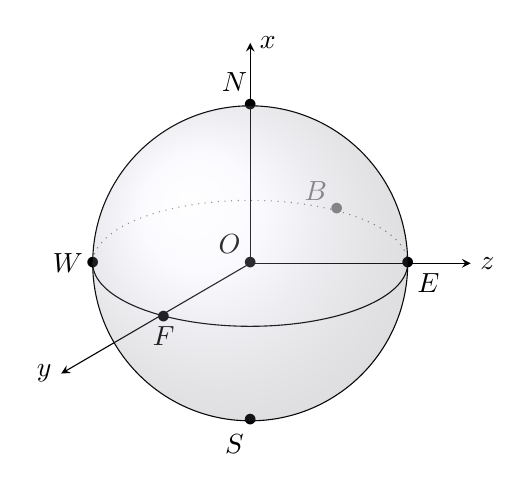
\begin{tikzpicture}[scale=2]
	\draw [samples=100,domain=-180:0] plot({cos(\x)},{0.4*sin(\x)});
	\draw [dotted, color=black!50, samples=100,domain=0:180] plot({cos(\x)},{0.4*sin(\x)});

	\draw  (0,0) node {$\bullet$} ;
	\draw  (0,0) node[above left] {$O$} ;
	\draw  (0,1) node {$\bullet$} ;
	\draw  (-0.1,1.15) node {$N$} ;
	\draw  (0,-1) node {$\bullet$} ;
	\draw  (-0.1,-1.15) node {$S$} ;
	\draw  (1,0) node {$\bullet$} ;
	\draw  (1,0) node[below right] {$E$} ;
	\draw  (-1,0) node {$\bullet$} ;
	\draw  (-1,0) node[left] {$W$} ;	
	\draw  (-0.55,-0.34) node {$\bullet$} ;
	\draw  (-0.55,-0.34) node[below] {$F$} ;	
	\draw  (0.55,0.34) node[color=black!50] {$\bullet$} ;
	\draw  (0.55,0.34) node[color=black!50, above left] {$B$} ;	
	
	\draw [>=stealth, ->] (0,0) -- (-1.2,-0.7) ;
	\draw  (-1.2,-0.7) node[left] {$y$} ;
	\draw [>=stealth, ->] (0,0) -- (0,1.4) ;
	\draw  (0,1.4) node[right] {$x$} ;
	\draw [>=stealth, ->] (0,0) -- (1.4,0) ;
	\draw  (1.4,0) node[right] {$z$} ;
	\draw (0,0) circle (1cm);
    \shade[ball color=blue!10!white,opacity=0.20] (0,0) circle (1cm);
\end{tikzpicture}
\end{center}
\caption{Sphère $\mathbb{S}_a^2$, points $N$, $S$, $E$, $W$, $F$ et $B$.}
\label{fig: sphere NSEWFB}
\end{figure}


Chacun des panels est délimité par quatre grands cercles (Voir Figure \ref{fig: panel I to VI}) :

\begin{itemize}
\item Le panel I est délimité par le cercle $C_V^1 = Vect(\mathbf{i}-\mathbf{j}, \mathbf{k}) \cap \mathbb{S}_a^2$ et le cercle $C_V^2 = Vect(\mathbf{i}+\mathbf{j}, \mathbf{k}) \cap \mathbb{S}_a^2$ ainsi que les cercles $C_{II}^1 = Vect(\mathbf{i}+\mathbf{k}, \mathbf{j}) \cap \mathbb{S}_a^2$ et $C_{II}^2 = Vect(\mathbf{i}-\mathbf{k}, \mathbf{j}) \cap \mathbb{S}_a^2$. Il ne contient que des points $\mathbf{x}=(x,y,z) \in \mathbb{S}_a^2 \subset \mathbb{R}^3$ vérifiant $x>0$. Le panel III est délimité par les mêmes cercles mais avec des points d'abscisse négative : $x<0$.
\item Le panel II est délimité par $C_V^2$ et $C_V^1$ ainsi que $C_I^1=Vect(\mathbf{j}+\mathbf{k},\mathbf{i}) \cap \mathbb{S}_a^2$ et $C_I^2=Vect(\mathbf{j}-\mathbf{k},\mathbf{i}) \cap \mathbb{S}_a^2$. Il est constitué de points $\mathbf{x} \in \mathbb{S}_a^2$ tels que $y>0$. Le panel IV est son symétrique, délimité par les mêmes cercles, avec $y<0$.
\item Le panel V est délimité par les cercles $C_I^1$, $C_I^2$, $C_{II}^1$ et $C_{II}^2$. Les points $\mathbf{x} = (x,y,z) \in \mathbb{S}_a^2$ qui le constituent sont tels que $z>0$. Son symétrique, le panel VI, est composé de points tels que $z<0$.


\end{itemize}

\begin{figure}[htbp]
\begin{center}
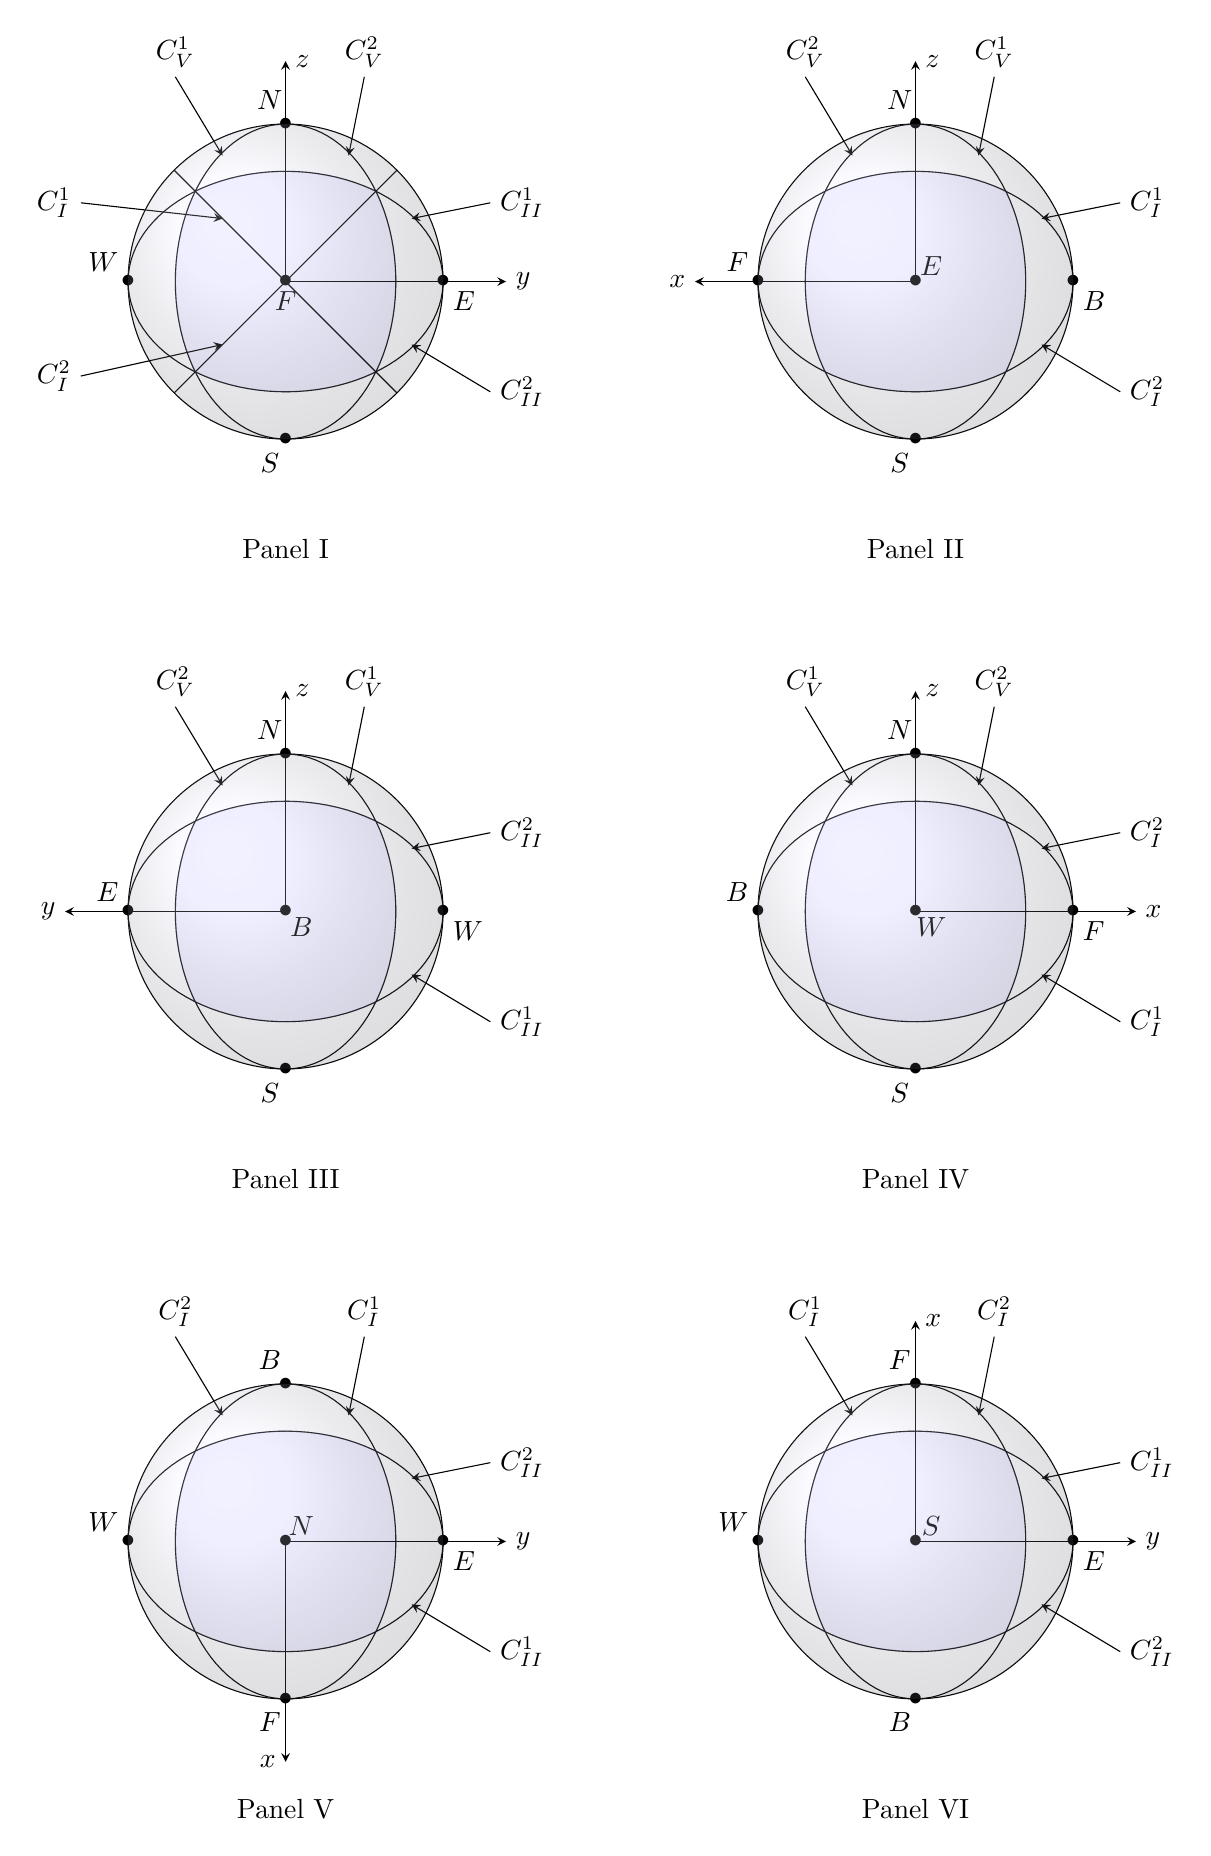
\begin{tikzpicture}[scale=2]
	%\draw [color=gray] (-1.5,-1.5) grid[step=0.1] (1.5,1.5);
	\draw [samples=100,domain=-180:180] plot({cos(\x)},{0.7*sin(\x)});
	\draw [samples=100,domain=180:-180] plot({0.7*cos(\x)},{sin(\x)}); 
	
	\filldraw[draw=black,fill=blue!30!white,opacity=0.20]
	plot [smooth,domain=-35:35] ({0.7*cos(\x)},{sin(\x)})
	-- plot [smooth,domain=55:125] ({cos(\x)},{0.7*sin(\x)})
	-- plot [smooth,domain=140:215] ({0.7*cos(\x)},{sin(\x)})
	-- plot [smooth,domain=230:305] ({cos(\x)},{0.7*sin(\x)})
	-- cycle;
	
	\draw (-0.707,0.707) -- (0.707,-0.707) ;
	\draw [>=stealth, <-] (-0.4,0.4) -- (-1.3,0.5) ;
	\draw  (-1.3,0.5) node[left] {$C_I^1$} ;
	\draw (-0.707,-0.707) -- (0.707,0.707) ;
	\draw [>=stealth, <-] (-0.4,-0.4) -- (-1.3,-0.6) ;
	\draw  (-1.3,-0.6) node[left] {$C_I^2$} ;
	
	\draw [>=stealth, ->] (0.5,1.3) -- (0.4,0.8) ;
	\draw  (0.5,1.3) node[above] {$C_V^2$} ;
	\draw [>=stealth, ->] (-0.7,1.3) -- (-0.4,0.8) ;
	\draw  (-0.7,1.3) node[above] {$C_V^1$} ;
	\draw [>=stealth, ->] (1.3,0.5) -- (0.8,0.4) ;
	\draw  (1.3,0.5) node[right] {$C_{II}^1$} ;
	\draw [>=stealth, ->] (1.3,-0.7) -- (0.8,-0.4) ;
	\draw  (1.3,-0.7) node[right] {$C_{II}^2$} ;
	
	\draw [>=stealth, ->] (0,0) -- (0,1.4) ;
	\draw  (0,1.4) node[right] {$z$} ;
	\draw [>=stealth, ->] (0,0) -- (1.4,0) ;
	\draw  (1.4,0) node[right] {$y$} ;
	
	\draw  (0,1) node {$\bullet$} ;
	\draw  (-0.1,1.15) node {$N$} ;
	\draw  (0,-1) node {$\bullet$} ;
	\draw  (-0.1,-1.15) node {$S$} ;
	\draw  (1,0) node {$\bullet$} ;
	\draw  (1,0) node[below right] {$E$} ;
	\draw  (-1,0) node {$\bullet$} ;
	\draw  (-1,0) node[above left] {$W$} ;
	\draw  (0,0) node {$\bullet$} ;
	\draw  (0,0) node[below] {$F$} ;
	
	\draw  (0,-1.7) node {Panel I} ;

	\draw (0,0) circle (1cm);
    \shade[ball color=blue!10!white,opacity=0.20] (0,0) circle (1cm);




	\draw [samples=100,domain=-180:180] plot({4+cos(\x)},{0.7*sin(\x)});
	\draw [samples=100,domain=180:-180] plot({4+0.7*cos(\x)},{sin(\x)}); 
	
	\filldraw[draw=black,fill=blue!30!white,opacity=0.20]
	plot [smooth,domain=-35:35] ({4+0.7*cos(\x)},{sin(\x)})
	-- plot [smooth,domain=55:125] ({4+cos(\x)},{0.7*sin(\x)})
	-- plot [smooth,domain=140:215] ({4+0.7*cos(\x)},{sin(\x)})
	-- plot [smooth,domain=230:305] ({4+cos(\x)},{0.7*sin(\x)})
	-- cycle;
	
	\draw [>=stealth, ->] (4.5,1.3) -- (4.4,0.8) ;
	\draw  (4.5,1.3) node[above] {$C_V^1$} ;
	\draw [>=stealth, ->] (3.3,1.3) -- (3.6,0.8) ;
	\draw  (3.3,1.3) node[above] {$C_V^2$} ;
	\draw [>=stealth, ->] (5.3,0.5) -- (4.8,0.4) ;
	\draw  (5.3,0.5) node[right] {$C_{I}^1$} ;
	\draw [>=stealth, ->] (5.3,-0.7) -- (4.8,-0.4) ;
	\draw  (5.3,-0.7) node[right] {$C_{I}^2$} ;
	
	\draw [>=stealth, ->] (4,0) -- (4,1.4) ;
	\draw  (4,1.4) node[right] {$z$} ;
	\draw [>=stealth, ->] (4,0) -- (4-1.4,0) ;
	\draw  (4-1.4,0) node[left] {$x$} ;
	
	\draw  (4,1) node {$\bullet$} ;
	\draw  (4-0.1,1.15) node {$N$} ;
	\draw  (4,-1) node {$\bullet$} ;
	\draw  (4-0.1,-1.15) node {$S$} ;
	\draw  (5,0) node {$\bullet$} ;
	\draw  (5,0) node[below right] {$B$} ;
	\draw  (4-1,0) node {$\bullet$} ;
	\draw  (4-1,0) node[above left] {$F$} ;
	\draw  (4,0) node {$\bullet$} ;
	\draw  (4.1,0.1) node {$E$} ;
	
	\draw  (4,-1.7) node {Panel II} ;

	\draw (4,0) circle (1cm);
    \shade[ball color=blue!10!white,opacity=0.20] (4,0) circle (1cm);






	\draw [samples=100,domain=-180:180] plot({cos(\x)},{-4+0.7*sin(\x)});
	\draw [samples=100,domain=180:-180] plot({0.7*cos(\x)},{-4+sin(\x)}); 
	
	\filldraw[draw=black,fill=blue!30!white,opacity=0.20]
	plot [smooth,domain=-35:35] ({0.7*cos(\x)},{-4+sin(\x)})
	-- plot [smooth,domain=55:125] ({cos(\x)},{-4+0.7*sin(\x)})
	-- plot [smooth,domain=140:215] ({0.7*cos(\x)},{-4+sin(\x)})
	-- plot [smooth,domain=230:305] ({cos(\x)},{-4+0.7*sin(\x)})
	-- cycle;
	
	\draw [>=stealth, ->] (0.5,-4+1.3) -- (0.4,-4+0.8) ;
	\draw  (0.5,-4+1.3) node[above] {$C_V^1$} ;
	\draw [>=stealth, ->] (-0.7,-4+1.3) -- (-0.4,-4+0.8) ;
	\draw  (-0.7,-4+1.3) node[above] {$C_V^2$} ;
	\draw [>=stealth, ->] (1.3,-4+0.5) -- (0.8,-4+0.4) ;
	\draw  (1.3,-4+0.5) node[right] {$C_{II}^2$} ;
	\draw [>=stealth, ->] (1.3,-4-0.7) -- (0.8,-4-0.4) ;
	\draw  (1.3,-4-0.7) node[right] {$C_{II}^1$} ;
	
	\draw [>=stealth, ->] (0,-4) -- (0,-4+1.4) ;
	\draw  (0,-4+1.4) node[right] {$z$} ;
	\draw [>=stealth, ->] (0,-4) -- (-1.4,-4) ;
	\draw  (-1.4,-4) node[left] {$y$} ;
	
	\draw  (0,-4+1) node {$\bullet$} ;
	\draw  (-0.1,-4+1.15) node {$N$} ;
	\draw  (0,-4-1) node {$\bullet$} ;
	\draw  (-0.1,-4-1.15) node {$S$} ;
	\draw  (1,-4) node {$\bullet$} ;
	\draw  (1,-4) node[below right] {$W$} ;
	\draw  (-1,-4) node {$\bullet$} ;
	\draw  (-1,-4) node[above left] {$E$} ;
	\draw  (0,-4) node {$\bullet$} ;
	\draw  (0.1,-4.1) node {$B$} ;
	
	\draw  (0,-4-1.7) node {Panel III} ;

	\draw (0,-4) circle (1cm);
    \shade[ball color=blue!10!white,opacity=0.20] (0,-4) circle (1cm);




	\draw [samples=100,domain=-180:180] plot({4+cos(\x)},{-4+0.7*sin(\x)});
	\draw [samples=100,domain=180:-180] plot({4+0.7*cos(\x)},{-4+sin(\x)}); 
	
	\filldraw[draw=black,fill=blue!30!white,opacity=0.20]
	plot [smooth,domain=-35:35] ({4+0.7*cos(\x)},{-4+sin(\x)})
	-- plot [smooth,domain=55:125] ({4+cos(\x)},{-4+0.7*sin(\x)})
	-- plot [smooth,domain=140:215] ({4+0.7*cos(\x)},{-4+sin(\x)})
	-- plot [smooth,domain=230:305] ({4+cos(\x)},{-4+0.7*sin(\x)})
	-- cycle;
	
	\draw [>=stealth, ->] (4+0.5,-4+1.3) -- (4+0.4,-4+0.8) ;
	\draw  (4+0.5,-4+1.3) node[above] {$C_V^2$} ;
	\draw [>=stealth, ->] (4-0.7,-4+1.3) -- (4-0.4,-4+.8) ;
	\draw  (4-0.7,-4+1.3) node[above] {$C_V^1$} ;
	\draw [>=stealth, ->] (4+1.3,-4+0.5) -- (4+0.8,-4+0.4) ;
	\draw  (4+1.3,-4+.5) node[right] {$C_{I}^2$} ;
	\draw [>=stealth, ->] (4+1.3,-4-0.7) -- (4+0.8,-4-0.4) ;
	\draw  (4+1.3,-4-0.7) node[right] {$C_{I}^1$} ;
	
	\draw [>=stealth, ->] (4,-4) -- (4,-4+1.4) ;
	\draw  (4,-4+1.4) node[right] {$z$} ;
	\draw [>=stealth, ->] (4,-4) -- (5.4,-4) ;
	\draw  (5.4,-4) node[right] {$x$} ;
	
	\draw  (4,-4+1) node {$\bullet$} ;
	\draw  (4-0.1,-4+1.15) node {$N$} ;
	\draw  (4,-4-1) node {$\bullet$} ;
	\draw  (4-0.1,-4-1.15) node {$S$} ;
	\draw  (5,-4) node {$\bullet$} ;
	\draw  (5,-4) node[below right] {$F$} ;
	\draw  (4-1,-4) node {$\bullet$} ;
	\draw  (4-1,-4) node[above left] {$B$} ;
	\draw  (4,-4) node {$\bullet$} ;
	\draw  (4.1,-4.1) node {$W$} ;
	
	\draw  (4,-4-1.7) node {Panel IV} ;

	\draw (4,-4) circle (1cm);
    \shade[ball color=blue!10!white,opacity=0.20] (4,-4) circle (1cm);




	\draw [samples=100,domain=-180:180] plot({cos(\x)},{-8+0.7*sin(\x)});
	\draw [samples=100,domain=180:-180] plot({0.7*cos(\x)},{-8+sin(\x)}); 
	
	\filldraw[draw=black,fill=blue!30!white,opacity=0.20]
	plot [smooth,domain=-35:35] ({0.7*cos(\x)},{-8+sin(\x)})
	-- plot [smooth,domain=55:125] ({cos(\x)},{0.7*sin(\x)-8})
	-- plot [smooth,domain=140:215] ({0.7*cos(\x)},{sin(\x)-8})
	-- plot [smooth,domain=230:305] ({cos(\x)},{0.7*sin(\x)-8})
	-- cycle;
	
	\draw [>=stealth, ->] (0.5,1.3-8) -- (0.4,0.8-8) ;
	\draw  (0.5,1.3-8) node[above] {$C_I^1$} ;
	\draw [>=stealth, ->] (-0.7,1.3-8) -- (-0.4,0.8-8) ;
	\draw  (-0.7,1.3-8) node[above] {$C_I^2$} ;
	\draw [>=stealth, ->] (1.3,0.5-8) -- (0.8,0.4-8) ;
	\draw  (1.3,0.5-8) node[right] {$C_{II}^2$} ;
	\draw [>=stealth, ->] (1.3,-0.7-8) -- (0.8,-0.4-8) ;
	\draw  (1.3,-0.7-8) node[right] {$C_{II}^1$} ;
	
	\draw [>=stealth, ->] (0,0-8) -- (0,-1.4-8) ;
	\draw  (0,-1.4-8) node[left] {$x$} ;
	\draw [>=stealth, ->] (0,0-8) -- (1.4,0-8) ;
	\draw  (1.4,0-8) node[right] {$y$} ;
	
	\draw  (0,1-8) node {$\bullet$} ;
	\draw  (-0.1,1.15-8) node {$B$} ;
	\draw  (0,-1-8) node {$\bullet$} ;
	\draw  (-0.1,-1.15-8) node {$F$} ;
	\draw  (1,0-8) node {$\bullet$} ;
	\draw  (1,0-8) node[below right] {$E$} ;
	\draw  (-1,0-8) node {$\bullet$} ;
	\draw  (-1,0-8) node[above left] {$W$} ;
	\draw  (0,0-8) node {$\bullet$} ;
	\draw  (0.1,0.1-8) node {$N$} ;
	
	\draw  (0,-1.7-8) node {Panel V} ;

	\draw (0,0-8) circle (1cm);
    \shade[ball color=blue!10!white,opacity=0.20] (0,0-8) circle (1cm);



	\draw [samples=100,domain=-180:180] plot({4+cos(\x)},{0.7*sin(\x)-8});
	\draw [samples=100,domain=180:-180] plot({4+0.7*cos(\x)},{sin(\x)-8}); 
	
	\filldraw[draw=black,fill=blue!30!white,opacity=0.20]
	plot [smooth,domain=-35:35] ({4+0.7*cos(\x)},{sin(\x)-8})
	-- plot [smooth,domain=55:125] ({4+cos(\x)},{0.7*sin(\x)-8})
	-- plot [smooth,domain=140:215] ({4+0.7*cos(\x)},{sin(\x)-8})
	-- plot [smooth,domain=230:305] ({4+cos(\x)},{0.7*sin(\x)-8})
	-- cycle;
	
	\draw [>=stealth, ->] (4+0.5,1.3-8) -- (4+0.4,0.8-8) ;
	\draw  (4+0.5,1.3-8) node[above] {$C_I^2$} ;
	\draw [>=stealth, ->] (4-0.7,1.3-8) -- (4-0.4,0.8-8) ;
	\draw  (4-0.7,1.3-8) node[above] {$C_I^1$} ;
	\draw [>=stealth, ->] (4+1.3,0.5-8) -- (4+0.8,0.4-8) ;
	\draw  (4+1.3,0.5-8) node[right] {$C_{II}^1$} ;
	\draw [>=stealth, ->] (4+1.3,-0.7-8) -- (4+0.8,-0.4-8) ;
	\draw  (4+1.3,-0.7-8) node[right] {$C_{II}^2$} ;
	
	\draw [>=stealth, ->] (4,0-8) -- (4,1.4-8) ;
	\draw  (4,1.4-8) node[right] {$x$} ;
	\draw [>=stealth, ->] (4,0-8) -- (4+1.4,0-8) ;
	\draw  (4+1.4,0-8) node[right] {$y$} ;
	
	\draw  (4,1-8) node {$\bullet$} ;
	\draw  (4-0.1,1.15-8) node {$F$} ;
	\draw  (4,-1-8) node {$\bullet$} ;
	\draw  (4-0.1,-1.15-8) node {$B$} ;
	\draw  (5,0-8) node {$\bullet$} ;
	\draw  (5,0-8) node[below right] {$E$} ;
	\draw  (4-1,0-8) node {$\bullet$} ;
	\draw  (4-1,0-8) node[above left] {$W$} ;
	\draw  (4,0-8) node {$\bullet$} ;
	\draw  (4+0.1,0.1-8) node {$S$} ;
	
	\draw  (4,-1.7-8) node {Panel VI} ;

	\draw (4,0-8) circle (1cm);
    \shade[ball color=blue!10!white,opacity=0.20] (4,0-8) circle (1cm);
\end{tikzpicture}
\end{center}
\caption{Délimitations des panels I à VI à l'aide des grands cercles}
\label{fig: panel I to VI}
\end{figure}




La grille Cubed-Sphere est constituée de l'intersection d'un ensemble de grands cercles pour chaque panel. On commence par introduire le système de coordonnées $(\xi,\eta)$ associés aux cercles centraux de chaque panel. $\xi$ et  $\eta$ sont définis comme il suit :

\begin{itemize}
\item Les courbes $\xi = 0$ et $\eta = 0$ sont les grands cercles de référence, notés respectivement $C_0^{(1)}$ et $C_0^{(2)}$ (en pointillés gras sur la Figure sur \ref{fig: panel I xi eta} et sur \ref{fig: panel I}). Pour le panel I, $C_0^{(1)}$ est le grand cercle passant par les points $N$ et $S$, il coupe orthogonalement $C_0^{(2)}$ qui est le grand cercle passant par $W$ et $E$,

\item $\xi$ est l'angle géodésique mesuré sur $C_0^{(2)}$ et $\eta$ l'angle géodésique mesuré sur $C_0^{(1)}$,

\item si $M$ est un point d'un panel, il est localisé de grâce aux angles géodésiques $\xi$ et $\eta$  (voir Figure \ref{fig: panel I xi eta}),

\item un panel est définit pour :
\begin{equation}
- \dfrac{\pi}{4} \leq \xi\text{, }\eta \leq \dfrac{\pi}{4},
\end{equation}

\item Soit $\mathbf{s}_{i,j}$ est un point du panel $K$, c'est un point du maillage si il est localisé grâce à ses coordonnées $(\xi_i, \eta_j)$ données par :
\begin{equation}
\xi_i = i \Delta \xi \text{ et } \eta_j = j \Delta \eta \text{ avec } -\dfrac{N}{2} \leq i,j \leq \dfrac{N}{2},
\end{equation}
dans ce qui suit, nous supposerons $N$ pair. $\Delta \xi$ et $\Delta \eta$ représentent le pas séparant régulièrement les grands les points dans le système de coordonnées $(\xi, \eta)$. 
\end{itemize}

Le cercle $C_0^{(2)}$ fait le tour de la sphère en formant un angle longitudinale de $2 \pi$, on peut donc insérer 4 panels notés $I$, $II$, $III$ et $IV$. De même, le long de $C_0^{(1)}$, sont présents les panels $I$, $V$, $III$ et $VI$.

\begin{figure}[htbp]
\begin{center}
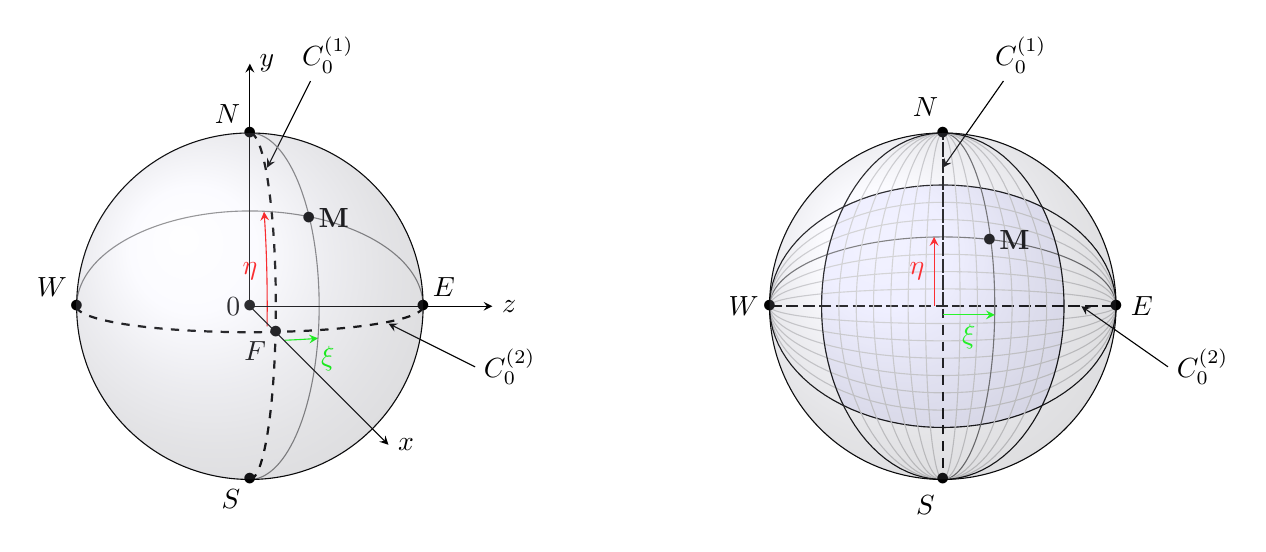
\begin{tikzpicture}[scale=2.2]
    \draw[>=stealth, ->, samples=100, color=green, domain=-79:-68] plot({1.05*cos(\x)},{0.2*sin(\x)});
    \draw[color=green] (.45,-.3) node{$\xi$} ;
    \draw[>=stealth, ->, samples=100, color=red, domain=-7:35] plot({0.1*cos(\x)},{0.95*sin(\x)});
    \draw[color=red] (0,0.2) node{$\eta$} ;

	\draw [dashed, line width=0.8pt, samples=100, domain=-180:0] plot({cos(\x)},{0.15*sin(\x)});
	\draw [dashed, line width=0.8pt, samples=100,domain=-90:90] plot({0.15*cos(\x)},{sin(\x)});
	\draw [>=stealth, ->] (1.3,-.35) -- (0.8,-0.1) ;
	\draw  (1.5,-.35) node {$C_0^{(2)}$} ;
	\draw [>=stealth, ->] (0.35,1.3) -- (0.1,0.8) ;
	\draw  (.45,1.45) node {$C_0^{(1)}$} ;
    
    
	\draw [samples=100, domain=-180:0, color=gray] plot({cos(\x)},{-0.55*sin(\x)});
	\draw [samples=100, domain=-90:90, color=gray] plot({0.4*cos(\x)},{sin(\x)});
	\draw (.34,0.51) node {$\bullet$} ;
	\draw (.34,0.51) node[right]{$\mathbf{M}$} ;
	
	\draw (1,0) node {$\bullet$} ;
	\draw (1,0) node[above right]{$E$} ;
	\draw (-1,0) node {$\bullet$} ;
	\draw (-1,0) node[above left]{$W$} ;
	\draw (0,1) node {$\bullet$} ;
	\draw (0,1) node[above left]{$N$} ;
	\draw (0,-1) node {$\bullet$} ;
	\draw (0,-1) node[below left]{$S$} ;
	\draw (.15,-0.15) node {$\bullet$} ;
	\draw (.15,-0.15) node[below left]{$F$} ;
	\draw (0,0) node {$\bullet$} ;
	\draw (0,0) node[left]{$0$} ;
	
	\draw [>=stealth, ->] (0,0) -- (0,1.4) ;
	\draw  (0,1.4) node[right] {$y$} ;
	\draw [>=stealth, ->] (0,0) -- (1.4,0) ;
	\draw  (1.4,0) node[right] {$z$} ;
	\draw [>=stealth, ->] (0,0) -- (.8,-0.8) ;
	\draw  (.8,-0.8) node[right] {$x$} ;
	
	
    \draw (0,0) circle (1cm);
    \shade[ball color=blue!10!white,opacity=0.20] (0,0) circle (1cm);
    
    
    
    
    
    
    \filldraw[draw=black,fill=blue!30!white,opacity=0.20]
	plot [smooth,domain=-35:35] ({4+0.7*cos(\x)},{sin(\x)})
	-- plot [smooth,domain=55:125] ({4+cos(\x)},{0.7*sin(\x)})
	-- plot [smooth,domain=140:215] ({4+0.7*cos(\x)},{sin(\x)})
	-- plot [smooth,domain=230:305] ({4+cos(\x)},{0.7*sin(\x)})
	-- cycle;	
	
	\draw [dashed, line width=0.8pt, samples=100,domain=180:-180] plot({4+cos(\x)},{0*sin(\x)});
	\draw [samples=100,domain=180:-180,color=gray!40] plot({4+cos(\x)},{0.1*sin(\x)});
	\draw [samples=100,domain=180:-180,color=gray!40] plot({4+cos(\x)},{0.2*sin(\x)});
	\draw [samples=100,domain=180:-180,color=gray!40] plot({4+cos(\x)},{0.3*sin(\x)});
	\draw [samples=100,domain=180:0,color=gray!120] plot({4+cos(\x)},{0.4*sin(\x)});
	\draw [samples=100,domain=0:-180,color=gray!40] plot({4+cos(\x)},{0.4*sin(\x)});
	\draw [samples=100,domain=180:-180,color=gray!40] plot({4+cos(\x)},{0.5*sin(\x)});
	\draw [samples=100,domain=180:-180,color=gray!40] plot({4+cos(\x)},{0.6*sin(\x)});
	\draw [samples=100,domain=180:-180] plot({4+cos(\x)},{0.7*sin(\x)});
	\draw [dashed, line width=0.8pt, samples=100,domain=180:-180] plot({4+0*cos(\x)},{sin(\x)});
	\draw [samples=100,domain=180:-180,color=gray!40] plot({4+0.1*cos(\x)},{sin(\x)});
	\draw [samples=100,domain=180:-180,color=gray!40] plot({4+0.2*cos(\x)},{sin(\x)});
	\draw [samples=100,domain=-90:90,color=gray!120] plot({4+0.3*cos(\x)},{sin(\x)});
	\draw [samples=100,domain=90:270,color=gray!40] plot({4+0.3*cos(\x)},{sin(\x)});
	\draw [samples=100,domain=180:-180,color=gray!40] plot({4+0.4*cos(\x)},{sin(\x)});
	\draw [samples=100,domain=180:-180,color=gray!40] plot({4+0.5*cos(\x)},{sin(\x)});
	\draw [samples=100,domain=180:-180,color=gray!40] plot({4+0.6*cos(\x)},{sin(\x)});
	\draw [samples=100,domain=180:-180] plot({4+0.7*cos(\x)},{sin(\x)}); 
	
	\draw [>=stealth, ->] (5.3,-.35) -- (4.8,-0) ;
	\draw  (5.5,-.35) node {$C_0^{(2)}$} ;
	\draw [>=stealth, ->] (4.35,1.3) -- (4,0.8) ;
	\draw  (4.45,1.45) node {$C_0^{(1)}$} ;
	\draw  (4,1) node {$\bullet$} ;
	\draw  (3.9,1.15) node {$N$} ;
	\draw  (4,-1) node {$\bullet$} ;
	\draw  (3.9,-1.15) node {$S$} ;
	\draw  (5,0) node {$\bullet$} ;
	\draw  (5.15,0) node {$E$} ;
	\draw  (3,0) node {$\bullet$} ;
	\draw  (4-1.15,0) node {$W$} ;
	
	\draw  (4.27,0.38) node {$\bullet$} ;
	\draw  (4.27,0.38) node[right] {$\mathbf{M}$} ;
	\draw [>=stealth, ->, color=green] (4,-0.05) -- (4.3,-0.05) ;
	\draw  (4.15,-0.05) node[color=green, below] {$\xi$} ;
	\draw [>=stealth, ->, color=red] (3.95,0) -- (3.95,0.4) ;
	\draw  (3.95,0.2) node[color=red, left] {$\eta$} ;

	\draw (4,0) circle (1cm);
    \shade[ball color=blue!10!white,opacity=0.20] (4,0) circle (1cm);  
   
\end{tikzpicture}
\end{center}
\caption{Sur un panel, un point $\mathbf{M}$ est localisé par $\xi$ et $\eta$.}
\label{fig: panel I xi eta}
\end{figure}


Dans ce cadre, on note $C^{(1)}_i$ le grand cercle obtenu par rotation de $C^{(1)}_0$ d'un angle géodésique $i \Delta \xi$ autour de l'axe $(Oz)$ et $C^{(2)}_j$ le cercle obtenu par rotation de $C^{(2)}_0$ d'angle $j \Delta \eta$ autour de $(Oy)$.

Le maillage associé au panel I est constitué des points d'intersection des $N+1$ cercles $( C_i^{(1)} )_{-N/2 \leq i \leq N/2}$ et des $N+1$ cercles $(C_j^{(2)})_{-N/2 \leq i \leq N/2}$ (Voir figure \ref{fig: panel I}). Il y a donc $(N+1)^2$ points d'intersection sur un panel.

\begin{figure}[htbp]
\begin{center}
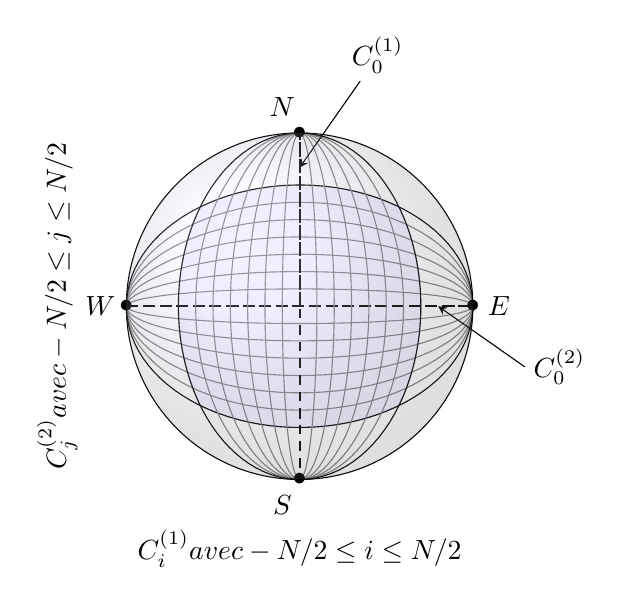
\begin{tikzpicture}[scale=2.2]
	%\draw [color=gray] (-2.5,-2.5) grid[step=0.1] (2.5,2.5);
	\filldraw[draw=black,fill=blue!30!white,opacity=0.20]
	plot [smooth,domain=-35:35] ({0.7*cos(\x)},{sin(\x)})
	-- plot [smooth,domain=55:125] ({cos(\x)},{0.7*sin(\x)})
	-- plot [smooth,domain=140:215] ({0.7*cos(\x)},{sin(\x)})
	-- plot [smooth,domain=230:305] ({cos(\x)},{0.7*sin(\x)})
	-- cycle;	
	
	\draw [dashed, line width=0.8pt, samples=100,domain=180:-180] plot({cos(\x)},{0*sin(\x)});
	\draw [samples=100,domain=180:-180,color=gray] plot({cos(\x)},{0.1*sin(\x)});
	\draw [samples=100,domain=180:-180,color=gray] plot({cos(\x)},{0.2*sin(\x)});
	\draw [samples=100,domain=180:-180,color=gray] plot({cos(\x)},{0.3*sin(\x)});
	\draw [samples=100,domain=180:-180,color=gray] plot({cos(\x)},{0.4*sin(\x)});
	\draw [samples=100,domain=180:-180,color=gray] plot({cos(\x)},{0.5*sin(\x)});
	\draw [samples=100,domain=180:-180,color=gray] plot({cos(\x)},{0.6*sin(\x)});
	\draw [samples=100,domain=180:-180] plot({cos(\x)},{0.7*sin(\x)});
	\draw [dashed, line width=0.8pt, samples=100,domain=180:-180] plot({0*cos(\x)},{sin(\x)});
	\draw [samples=100,domain=180:-180,color=gray] plot({0.1*cos(\x)},{sin(\x)});
	\draw [samples=100,domain=180:-180,color=gray] plot({0.2*cos(\x)},{sin(\x)});
	\draw [samples=100,domain=180:-180,color=gray] plot({0.3*cos(\x)},{sin(\x)});
	\draw [samples=100,domain=180:-180,color=gray] plot({0.4*cos(\x)},{sin(\x)});
	\draw [samples=100,domain=180:-180,color=gray] plot({0.5*cos(\x)},{sin(\x)});
	\draw [samples=100,domain=180:-180,color=gray] plot({0.6*cos(\x)},{sin(\x)});
	\draw [samples=100,domain=180:-180] plot({0.7*cos(\x)},{sin(\x)}); 
	
	\draw [>=stealth, ->] (1.3,-.35) -- (0.8,-0) ;
	\draw  (1.5,-.35) node {$C_0^{(2)}$} ;
	\draw [>=stealth, ->] (0.35,1.3) -- (0,0.8) ;
	\draw  (0.45,1.45) node {$C_0^{(1)}$} ;
	\draw  (0,1) node {$\bullet$} ;
	\draw  (-0.1,1.15) node {$N$} ;
	\draw  (0,-1) node {$\bullet$} ;
	\draw  (-0.1,-1.15) node {$S$} ;
	\draw  (1,0) node {$\bullet$} ;
	\draw  (1.15,0) node {$E$} ;
	\draw  (-1,0) node {$\bullet$} ;
	\draw  (-1.15,0) node {$W$} ;

	\draw (0,0) circle (1cm);
    \shade[ball color=blue!10!white,opacity=0.20] (0,0) circle (1cm);
    
    \draw  (-1.4,0) node[rotate=90] {$ C_j^{(2)}\text{ avec }-N/2\leq j \leq N/2$} ;
    \draw  (0,-1.4) node {$ C_i^{(1)}\text{ avec }-N/2\leq i \leq N/2$} ;

\end{tikzpicture}
\end{center}
\caption{Le panel I est constitué des points d'intersection d'un ensemble de grands cercles.}
\label{fig: panel I}
\end{figure}  

En reproduisant le procédé pour chaque panel, on constitue la Cubed-Sphere associée à la base $(\mathbf{i},\mathbf{j},\mathbf{k})$ et de paramètre $N$.

\begin{definition}
La Cubed-Sphere est une grille de la sphère $\mathbb{S}_a^2$. Elle est constituée d'une partition de la sphère en 6 panels identiques notés panel I (Front), II (East), III (Bottom), IV (West), V (North) et VI (South). Chaque panel est équipé de son propre système de coordonnées :
\begin{equation}
\left( \xi^{(k)}, \eta^{(k)} \right) \text{, } -\dfrac{\pi}{4} \leq \xi^{(k)}, \eta^{(k)} \leq \dfrac{\pi}{4} \text{, } I \leq k \leq VI.
\end{equation}
Les points de la Cubed-Sphère sont notés $\mathbf{s}_{i,j}^{(k)}$. Ils ont pour coordonnées $\left( \xi_i^{(k)}, \eta_j^{(k)}  \right)$ avec :
\begin{equation}
\xi_i^{(k)} = i \Delta \xi \text{, } \eta_j^{(k)} = j \Delta \eta \text{, } -N/2 \leq i, j \leq N/2 \text{ et } I \leq k \leq VI,
\end{equation}
où le pas de discrétisation est :
\begin{equation}
\Delta \xi = \Delta \eta = \dfrac{\pi}{2 N}.
\end{equation}
\end{definition}

Les points $\mathbf{s}_{i,j}^{(k)}$ de chaque panel se divisent en 3 catégories :
\begin{itemize}
\item Les points intérieurs si :
\begin{equation}
- \dfrac{N}{2}+1 \leq i,j \leq \dfrac{N}{2}-1
\end{equation}
Ils sont au nombre de $(N-1)^2$ par panel.
\item Les $4(N-1)$ points de bords de chaque panel, si :
\begin{equation}
\left[ j=\pm \dfrac{N}{2} \text{ et } - \dfrac{N}{2}+1 \leq i \leq \dfrac{N}{2}-1 \right] \text{ ou } \left[ i=\pm \dfrac{N}{2} \text{ et } - \dfrac{N}{2}+1 \leq j \leq \dfrac{N}{2}-1 \right]
\end{equation}
\item Les $4$ points de coins si :
\begin{equation}
i, j = \pm \dfrac{N}{2}
\end{equation}
\end{itemize}

\begin{proposition}
La Cubed-Sphere est composée de $6N^2 +2$ points.
\end{proposition}

\begin{proof}
Il y a 6 intérieurs de panels de $(N-1)^2$ points, 12 arrêtes de $N-1$ points et 8 sommets. Ainsi le nombre de points sur la Cubed-Sphere est :
$$
6 (N-1)^2 + 12 (N-1)+8=6N^2+2
$$
\end{proof}











\section{Coordonnées Gnomoniques}

On considère un cube inscrit dans la Sphère $\mathbb{S}_a^2$. Le demi côté de ce cube mesure $R=\frac{\sqrt{3}}{6}a$. Chaque face du cube est donnée par :
\begin{itemize}
\item la face centrée sur $F'=(R,0,0)$ : 
\begin{equation}
\left\lbrace
\mathbf{x}' = (R,y',z') \in \mathbb{R}^3 \text{ tels que } -R  \leq y',z' \leq R
\right\rbrace
\end{equation}

\item la face centrée sur $B'=(-R,0,0)$ : 
\begin{equation}
\left\lbrace
\mathbf{x}' = (-R,y',z') \in \mathbb{R}^3 \text{ tels que } -R  \leq y',z' \leq R
\right\rbrace
\end{equation}

\item la face centrée sur $E'=(0,R,0)$ : 
\begin{equation}
\left\lbrace
\mathbf{x}' = (x',R,z') \in \mathbb{R}^3 \text{ tels que } -R  \leq x',z' \leq R
\right\rbrace
\end{equation}

\item la face centrée sur $W'=(0,-R,0)$ : 
\begin{equation}
\left\lbrace
\mathbf{x}' = (x',-R,z') \in \mathbb{R}^3 \text{ tels que } -R  \leq x',z' \leq R
\right\rbrace
\end{equation}

\item la face centrée sur $N'=(0,0,R)$ : 
\begin{equation}
\left\lbrace
\mathbf{x}' = (x',y',R) \in \mathbb{R}^3 \text{ tels que } -R  \leq x',y' \leq R
\right\rbrace
\end{equation}

\item la face centrée sur $S'=(0,0,-R)$ : 
\begin{equation}
\left\lbrace
\mathbf{x}' = (x',y',-R) \in \mathbb{R}^3 \text{ tels que } -R  \leq x',y' \leq R
\right\rbrace
\end{equation}
\end{itemize}

$F$ est la projection gnomonique de $F'$ sur la sphère $\mathbb{S}_a^2$, $E$ celle de $E'$, ...
Si l'on considère par exemple le panel I, un point $\mathbf{M'}=(x',y',z')$ de la face centré sur $F'$ est projeté en $\mathbf{M} = (x,y,z)$ un point du panel I (Voir figure \ref{fig: projection gnomonique}).

\begin{figure}[htbp]
\begin{center}
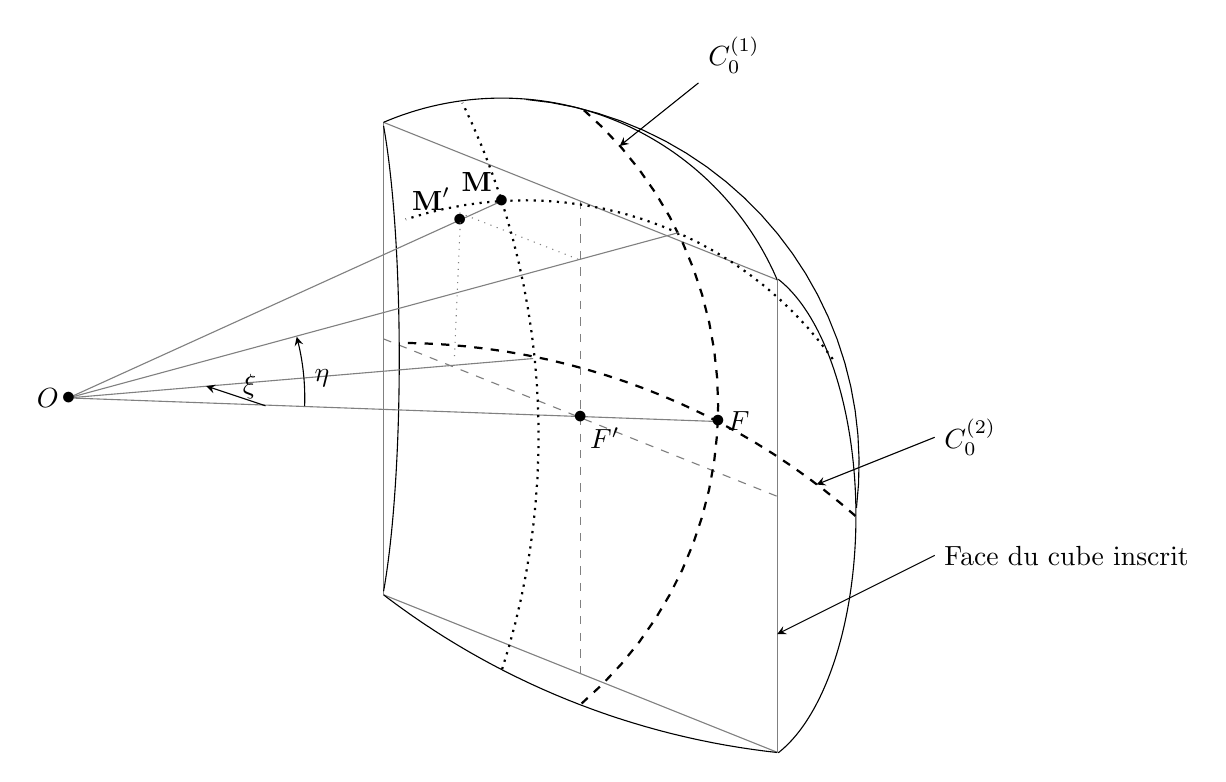
\begin{tikzpicture}[scale=1]
	\draw [color=gray] (0,3) -- (0,-3) ;
	\draw [color=gray] (0,-3) -- (5,-5) ;
	\draw [color=gray] (5,-5) -- (5,1) ;
	\draw [color=gray] (5,1) -- (0,3) ;
	\draw [dashed, color=gray] (0,.25) -- (5,-1.75) ;
	\draw [dashed, color=gray] (2.5,2) -- (2.5,-4) ;
	
	\draw [samples=100,domain=-70:70] plot({4.5+1.5*cos(\x)},{-2+3.2*sin(\x)});
	\draw [samples=100,domain=-53:53] plot({-0.3+0.5*cos(\x)},{3.7*sin(\x)});
	\draw [samples=100,domain=113.2:23.2] plot({1.5+sqrt(14.5)*cos(\x)},{-.5+sqrt(14.5)*sin(\x)});
	\draw [samples=100,domain=-96.24:-127.41] plot({6.09+sqrt(100.46)*cos(\x)},{4.96+sqrt(100.46)*sin(\x)});
	
	\draw [shift={(1.39,-1.34)}] plot[domain=-0.12:1.48,variable=\t]({1*4.65*cos(\t r)+0*4.65*sin(\t r)},{0*4.65*cos(\t r)+1*4.65*sin(\t r)});
	
	
	\draw [color=gray] (-4,-.5) -- (4.25,-0.8) ;
	\draw  (2.5,-.75) node {$\bullet$} ;
	\draw  (2.5,-.75) node[below right] {$F'$} ;
	\draw  (4.25,-0.8) node {$\bullet$} ;
	\draw  (4.25,-0.8) node[right] {$F$} ;
	
	\draw [dashed, line width=0.8pt, shift={(-0.74,-0.6)}] plot[domain=-0.86:0.86,variable=\t]({1*4.99*cos(\t r)+0*4.99*sin(\t r)},{0*4.99*cos(\t r)+1*4.99*sin(\t r)});
	\draw [dashed, line width=0.8pt, shift={(0.16,-8.64)}] plot[domain=0.85:1.56,variable=\t]({1*8.84*cos(\t r)+0*8.84*sin(\t r)},{0*8.84*cos(\t r)+1*8.84*sin(\t r)});
	
	\draw [color=gray] (-4,-.5) -- (1.5,2) ;
	\draw  (1.5,2) node {$\bullet$} ;
	\draw  (1.5,2) node[above left] {$\textbf{M}$} ;
	
	\draw [dotted, line width=0.8pt, shift={(1.79,-2.8)}] plot[domain=0.62:1.89,variable=\t]({1*4.81*cos(\t r)+0*4.81*sin(\t r)},{0*4.81*cos(\t r)+1*4.81*sin(\t r)});
	\draw [dotted, line width=0.8pt, shift={(-7.75,-0.98)}] plot[domain=-0.31:0.45,variable=\t]({1*9.72*cos(\t r)+0*9.72*sin(\t r)},{0*9.72*cos(\t r)+1*9.72*sin(\t r)});

	\draw [color=gray] (-4,-.5) -- (1.9,0) ;
	\draw [color=gray] (-4,-.5) -- (3.75,1.6) ;
	
	\draw  (.97,1.75) node {$\bullet$} ;
	\draw  (.97,1.75) node[above left] {$\textbf{M}'$} ;
	\draw [dotted, color=gray] (.965,1.85) -- (2.5,1.25) ;
	\draw [dotted, color=gray] (.975,1.73) -- (.9,0) ;
	
	\draw  (-4,-.5) node {$\bullet$} ;
	\draw  (-4,-.5) node[left] {$O$} ;
	
	\draw [>=stealth, ->] (-1.5,-.6) -- (-2.25,-.35) ;
	\draw  (-1.7,-.35) node {$\xi$} ;
	\draw [>=stealth, ->,domain=-2:15] plot({-4+3*cos(\x)},{-.5+3*sin(\x)});
	\draw  (-1,-.25) node[right] {$\eta$} ;
	
	\draw [>=stealth, <-] (5.5,-1.6) -- (7,-1) ;
	\draw  (7,-1) node[right] {$C_0^{(2)}$} ;
	\draw [>=stealth, <-] (3,2.7) -- (4,3.5) ;
	\draw  (4,3.5) node[above right] {$C_0^{(1)}$} ;
	\draw [>=stealth, <-] (5,-3.5) -- (7,-2.5) ;
	\draw  (7,-2.5) node[right] {Face du cube inscrit} ;

\end{tikzpicture}
\end{center}
\caption{Projection gnomonique.}
\label{fig: projection gnomonique}
\end{figure}  

On constate alors les relations suivantes :
\begin{equation}
\tan \xi = \dfrac{y'}{x'} = \dfrac{y}{x} \text{ et } \tan \eta = \dfrac{z'}{x'} = \dfrac{z}{x}
\end{equation}

Or $\mathbf{M}'$ est un point de la face du cube centrée en $\mathbf{M}'$, donc $x'=R=\frac{\sqrt{3}}{6}a$ :
\begin{equation}
\tan \xi = \dfrac{y'}{R} = \dfrac{y}{x} \text{ et } \tan \eta = \dfrac{z'}{R} = \dfrac{z}{x}
\end{equation}

Quel que soit la face, on pose $(X,Y)$ les coordonnées gnomoniques:
\begin{equation}
X:=\tan \xi \text{ et } Y:= \tan \eta
\end{equation}

Un point de la sphère est localisé de manière unique par sa face et ses coordonnées gnomoniques. Si on se donne $(X,Y)$ un couple de coordonnées gnomoniques du panel I, on a :

\begin{equation}
\left\lbrace
\begin{array}{rcl}
x^2+y^2+z^2 & = & a^2\\
X & = & \dfrac{y}{x} \\
Y & = & \dfrac{z}{x}
\end{array}
\right.
\end{equation}

ainsi $x^2 \left( 1+X^2+Y^2 \right) = a^2$, d'où :

\begin{equation}
\left\lbrace
\begin{array}{rclcl}
x & = & \pm \dfrac{a}{\sqrt{1+X^2+Y^2}}& = & \dfrac{a}{\sqrt{1+X^2+Y^2}}\\
y & = & xX &&\\
z & = & xY &&
\end{array}
\right.
\end{equation}

le signe de $x$ est donné car $\mathbf{x}$ est un point du panel I qui ne contient que des points d'abscisse positive.

De là, on peut dériver chaque donnée :

\begin{equation}
\dfrac{\partial y}{\partial \xi} = \dfrac{\partial x}{\partial \xi} X + x \dfrac{\partial X}{\partial \xi} = \dfrac{\partial x}{\partial \xi} X + x(1+X^2)
\end{equation}

\begin{equation}
\dfrac{\partial z}{\partial \xi} = \dfrac{\partial x}{\partial \xi} Y + x \dfrac{\partial Y}{\partial \xi} = \dfrac{\partial x}{\partial \xi} Y
\end{equation}

Le calcul de ces dérivées dépend de $\dfrac{\partial x}{\partial \xi}$ :

\begin{equation*}
\begin{array}{rcl}
0 & = & \dfrac{\partial}{\partial \xi} ( x^2+y^2+z^2) \\
  & = & 2x\dfrac{\partial x}{\partial \xi} + 2y\dfrac{\partial y}{\partial \xi}+ 2z\dfrac{\partial z}{\partial \xi} \\
  & = & x \dfrac{\partial x}{\partial \xi} ( 1 +X^2 + Y^2) + x^2 X (1+X^2)
\end{array}
\end{equation*}

d'où, en posant $\delta = \sqrt{1+X^2+Y^2}$, sur le panel I :

\begin{equation}
\left\lbrace
\begin{array}{rcl}
\dfrac{\partial x}{\partial \xi} & = & -\dfrac{y(1+X^2)}{\delta^2}\\
\dfrac{\partial y}{\partial \xi} & = & x \dfrac{1+X^2}{\delta^2} (1+Y^2)\\
\dfrac{\partial z}{\partial \xi} & = & - \dfrac{yY(1+X^2)}{\delta^2}
\end{array}
\right.
\end{equation}

De la même manière, on a sur le panel I :

\begin{equation}
\left\lbrace
\begin{array}{rcl}
\dfrac{\partial x}{\partial \eta} & = & - z\dfrac{1+Y^2}{\delta^2}\\
\dfrac{\partial y}{\partial \eta} & = & - zX\dfrac{1+Y^2}{\delta^2}\\
\dfrac{\partial z}{\partial \eta} & = & - x(1+X^2) \dfrac{1+Y^2}{\delta^2}
\end{array}
\right.
\end{equation}

On en déduit la base sur le panel I $\left( \mathbf{g}_{\xi}, \mathbf{g}_{\eta} \right)$ donnée par :

\begin{equation}
\mathbf{g}_{\xi} = \dfrac{1+X^2}{\delta^2} \begin{pmatrix}
-y \\ x(1+Y^2) \\ -yY
\end{pmatrix} \text{ et } \mathbf{g}_{\eta} = \dfrac{1+Y^2}{\delta^2} \begin{pmatrix}
-z \\ -zX \\ x(1+X^2)
\end{pmatrix}
\label{eq: base locale I}
\end{equation}

Des calculs similaires peuvent être effectuées sur les autres panels. Les résultats sont donnés dans le tableau \ref{tab: base g_xi g_eta}.

\begin{table}[htbp]
\begin{center}
\begin{equation*}
\begin{array}{|c|c|}
\hline
\textbf{Panel} & \textbf{Base } \left( \mathbf{g}_{\xi}, \mathbf{g}_{\eta} \right)\\

\hline
\hline
I & \mathbf{g}_{\xi} = \dfrac{1+X^2}{\delta^2} \begin{pmatrix}
-y \\ x(1+Y^2) \\ -yY
\end{pmatrix} \text{ et } \mathbf{g}_{\eta} = \dfrac{1+Y^2}{\delta^2} \begin{pmatrix}
-z \\ -zX \\ x(1+X^2)
\end{pmatrix} \\

\hline
II & \mathbf{g}_{\xi} = \dfrac{1+X^2}{\delta^2} \begin{pmatrix}
-y(1+Y^2) \\ x \\ xY
\end{pmatrix} \text{ et } \mathbf{g}_{\eta} = \dfrac{1+Y^2}{\delta^2} \begin{pmatrix}
zX \\ -z \\ y(1+X^2)
\end{pmatrix} \\

\hline
III & \mathbf{g}_{\xi} = \dfrac{1+X^2}{\delta^2} \begin{pmatrix}
-y \\ x(1+Y^2) \\ yY
\end{pmatrix} \text{ et } \mathbf{g}_{\eta} = \dfrac{1+Y^2}{\delta^2} \begin{pmatrix}
-z \\ -zX \\ x(1+X^2)
\end{pmatrix} \\

\hline
IV & \mathbf{g}_{\xi} = \dfrac{1+X^2}{\delta^2} \begin{pmatrix}
-y(1+Y^2) \\ x \\ -xY
\end{pmatrix} \text{ et } \mathbf{g}_{\eta} = \dfrac{1+Y^2}{\delta^2} \begin{pmatrix}
-zX \\ z \\ -y(1+X^2)
\end{pmatrix} \\

\hline
V & \mathbf{g}_{\xi} = \dfrac{1+X^2}{\delta^2} \begin{pmatrix}
-yY \\ z(1+Y^2) \\ -y
\end{pmatrix} \text{ et } \mathbf{g}_{\eta} = \dfrac{1+Y^2}{\delta^2} \begin{pmatrix}
-z(1+X^2) \\ xX \\ x
\end{pmatrix} \\

\hline
VI & \mathbf{g}_{\xi} = \dfrac{1+X^2}{\delta^2} \begin{pmatrix}
-yY \\ -z(1+Y^2) \\ y
\end{pmatrix} \text{ et } \mathbf{g}_{\eta} = \dfrac{1+Y^2}{\delta^2} \begin{pmatrix}
-z(1+X^2) \\ -xX \\ x
\end{pmatrix}\\
\hline

\end{array}
\end{equation*}
\end{center}
\caption{Bases $\left( \mathbf{g}_{\xi}, \mathbf{g}_{\eta} \right)$ sur chaque panel.}
\label{tab: base g_xi g_eta}
\end{table}
















\section{Calcul intrinsèque sur la Cubed-Sphère}


















